\documentclass{article}

\usepackage[utf8]{inputenc}
\usepackage{amsthm}
\usepackage{amssymb}
\usepackage{mathtools}
\usepackage{graphicx}
\usepackage{mdframed}
\usepackage{float}
\usepackage[top=0.75in, bottom=0.75in, left=0.75in, right=0.75in]{geometry}
\usepackage{gauss}

\usepackage{array}
\allowdisplaybreaks

\makeatletter
\newcounter{elimination@steps}
\newcolumntype{R}[1]{>{\raggedleft\arraybackslash$}p{#1}<{$}}
\def\elimination@num@rights{}
\def\elimination@num@variables{}
\def\elimination@col@width{}
\newenvironment{elimination}[4][0]
{
    \setcounter{elimination@steps}{0}
    \def\elimination@num@rights{#1}
    \def\elimination@num@variables{#2}
    \def\elimination@col@width{#3}
    \renewcommand{\arraystretch}{#4}
    \start@align\@ne\st@rredtrue\m@ne
}
{
    \endalign
    \ignorespacesafterend
}
\newcommand{\step}[2]
{
    \ifnum\value{elimination@steps}>0\sim\quad\fi
    \left[
        \ifnum\elimination@num@rights>0
            \begin{array}
            {@{}*{\elimination@num@variables}{R{\elimination@col@width}}
            |@{}*{\elimination@num@rights}{R{\elimination@col@width}}}
        \else
            \begin{array}
            {@{}*{\elimination@num@variables}{R{\elimination@col@width}}}
        \fi
            #1
        \end{array}
    \right]
    & 
    \begin{array}{l}
        #2
    \end{array}
    \addtocounter{elimination@steps}{1}
}
\makeatother

\DeclarePairedDelimiter{\abs}{\lvert}{\rvert}
\DeclarePairedDelimiter{\norm}{\lvert \lvert}{\rvert \rvert}

\newtheoremstyle{break}% name
  {}%         Space above, empty = `usual value'
  {}%         Space below
  {\itshape}% Body font
  {}%         Indent amount (empty = no indent, \parindent = para indent)
  {\bfseries}% Thm head font
  {.}%        Punctuation after thm head
  {\newline}% Space after thm head: \newline = linebreak
  {}%         Thm head spec

\newtheorem{Def}{Definition}[section]

\theoremstyle{break}

\newtheorem{innerEx}{Exempel}[section]
\newtheorem{sats}{Sats}[section]
\newtheorem{Rem}{Anmärkning}[]

\newenvironment{Ex}
{\begin{mdframed} \begin{innerEx} \vspace{3pt}}
{\vspace{3pt} \end{innerEx} \end{mdframed}}  

\newenvironment{bevis}
{\begin{mdframed} \begin{proof} \vspace{3pt}}
{\vspace{3pt} \end{proof} \end{mdframed}}


\title{
	 Linjär Algebra\\
	 Föreläsning 10
    \author{Erik Sjöström}
}
\begin{document}
\maketitle
\section{System av linjär ekvationer} % (fold)
\label{sec:system_av_linj_r_ekvationer}
Ett system av linjära ekvationer med \textit{n} obekanta skrivs på detta sätt:
\[
\left\{ \begin{array}{ccccccccc}
	a_{11}x_1 &+& a_{12}x_2 &+ &...& +& a_{1n}x_n &=& b_1\\
	a_{21}x_1 &+& a_{22}x_2 &+ &...& +& a_{2n}x_n &=& b_2\\
	\vdots && \vdots && \vdots && \vdots && \vdots       \\
	a_{m1}x_1 &+& a_{m2}x_2 &+&...&+& a_{mn}x_n &=& b_m 
\end{array}
\]
Där $a_{ij}$, $b_j$ är reella tal och $x_j$ är obekant.\\
Man söker en lösning sådan att alla ekvationer är uppfyllda samtidigt.\\
Med matris-vektor beteckning skrivs ekvationssystemet som:
\[
\overbrace{
\begin{bmatrix}
a_{11}&a_{12}&...&a_{1n}\\
a_{21}&a_{22}&...&a_{2n}\\
\vdots & \vdots &\ddots& \vdots\\
a_{m1}&a_{m2}&...&a_{mn} \end{bmatrix}}^\text{Koefficientmatris} \cdot \overbrace{\begin{bmatrix} x_1\\x_2\\\vdots\\x_n \end{bmatrix}}^\text{Obekanta} = \overbrace{\begin{bmatrix} b_1\\b_2\\\vdots\\b_m \end{bmatrix}}^\text{Högerled}
\] 
Två fundamentala frågor:
\begin{enumerate}
	\item Finns det en lösning? (Existens)
	\item Om det finns en lösning, finns det flera? (Entydighet)
\end{enumerate}

\begin{Ex}
    \[
        \begin{cases}
        	x_1 - 2x_2 = -1 &\text{Två ekvationer}\\ 
        	-x_1 + 3x_2 = 3 &\text{Två obekanta}
        \end{cases}
    \]
    Dessa två ekvationer kan tolkas som två linjer:
    \begin{align*}
    &x_2 = \frac{x_1 + 1}{2} = l_1 & x_1 = 3x_2 -3 = l_2
    \end{align*}
    \begin{center}
    	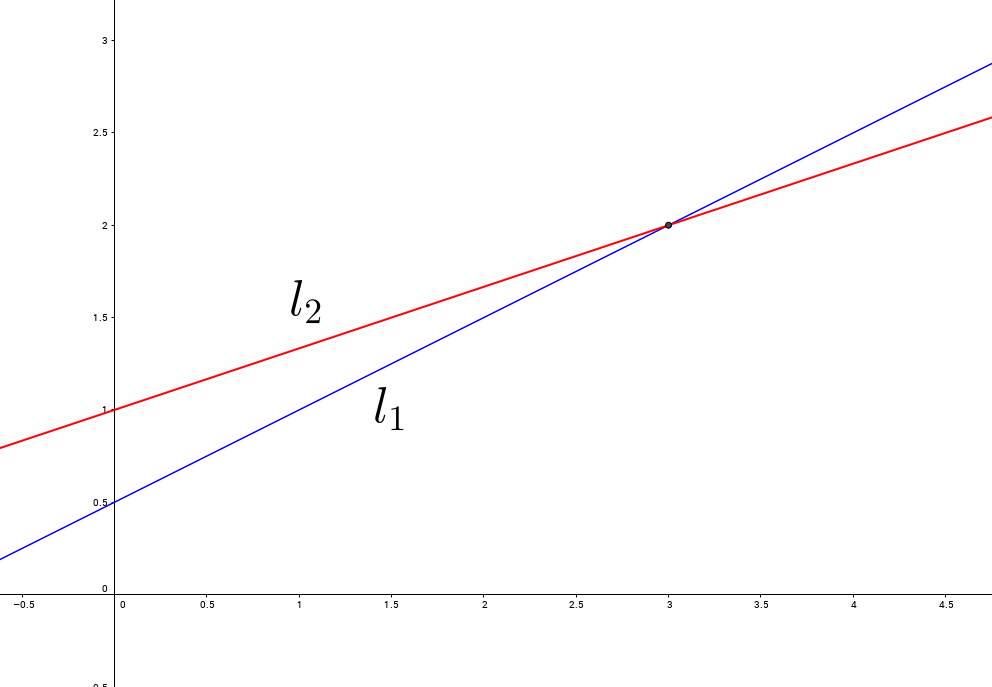
\includegraphics[scale=0.4]{skarning.png}
    \end{center}
    Lösningen ges av skärningen mellan linjerna:
    \[
        \begin{bmatrix} x_1\\x_2 \end{bmatrix} = \begin{bmatrix} 3\\2 \end{bmatrix}
    \]
    Det finns inga fler lösningar eftersom det bara finns en skärningspunkt.
\end{Ex}
% section system_av_linj_r_ekvationer (end)
\section{$\mathbb{R}^n$} % (fold)
\label{sec: R^n}
I $\mathbb{R}^n$ kan vi ej rita linjer!\\
Det allmänna tillvägagångssättet är att bestämma en lösning med Gauseliminering på totalmatrisen som består av.
\[
    \begin{bmatrix}
    \begin{array}{c|c}
    	\mathbf{A} & \vec{b}
    \end{array}
    \end{bmatrix}
\]
Där \textbf{A} är koefficientmatrisen och $\vec{b}$ är högerledet.
Tillåtna elementära radoperationer i gauseliminering är:
\begin{itemize}
	\item Addition: Addera till en rad en multipel av en annan rad
	\item Platsbyte: Låt två rader byta plats
	\item Skalning: Multiplicera en rad med en konstant $\neq 0$
\end{itemize}
Dessa operationer bibehåller lösningsmängden.
\newpage
\begin{Ex}
    \[
        \begin{cases}
        	x_1 - 2x_2 = -1 &\text{Två ekvationer}\\ 
        	-x_1 + 3x_2 = 3 &\text{Två obekanta}
        \end{cases}
    \]
    Med matris-vektor beteckning:
    \[
        \begin{bmatrix} 1&-2\\-1&3 \end{bmatrix} \cdot \begin{bmatrix} x_1\\x_2 \end{bmatrix} = \begin{bmatrix} -1\\3 \end{bmatrix}
    \]
    Och om vi nu skriver om det som totalmatrisen ovan:
    \[
    \begin{bmatrix}
    \begin{array}{cc|c}
    1 & -2 & -1 \\
    -1 & 3 & 3
    \end{array}
    \end{bmatrix}
    \]
    Vi vill ha noll i det nedre vänstra hörnet. Så vi använder additionsoperationen, och adderar rad 1 till rad 2:
    \begin{elimination}[1]{2}{1.75em}{1.1}
    \step
    {
        1 & -2 & -1\\
        -1 & 3 & 3
    }
    {
               \\
        +R_{1} \\
    }
    \step
    {
        1 & -2 & -1\\
        0 & 1 & 2
    }
    {
                \\
                \\
    }
\end{elimination}
\noindent
Nu vill vi sätta det första elementet i den andra kolumnen (\textit{-2}) till 0. Det gör vi genom att kombinera skalnings- och additions-operationen. Vi adderar alltså 2 $\cdot$ Rad 2 till Rad 1.
\begin{elimination}[1]{2}{1.75em}{1.1}
\step
{
    1 & -2 & -1 \\
    0 & 1 & 2
}
{
    + 2 \cdot R_2\\
    \\
}
\step
{
    1 & 0 & 3\\
    0 & 1 & 2
}
{
    \\
    \\
}
\end{elimination}
Om vi nu stoppar tillbaka det i ekvationssystemet får vi:
\[
    \begin{cases}
        1x_1 + 0x_2 = 3 \\
        0x_1 + 1x_2 = 2
    \end{cases}
\]
Dvs:
\[
    \begin{cases}
        x_1 = 3\\
        x_2 = 2
    \end{cases}
\]
Vi har nu löst ekvationssystemet med gauseliminering och:
    \[
    \begin{bmatrix}
    \begin{array}{cc|c}
    1 & 0 & 3\\
    0 & 1 & 2
    \end{array}
    \end{bmatrix}
    \]
    Är skriven på reducerad trappstegsform.
\end{Ex}

\begin{Rem}
    Man använder '$\sim$' för att marker att matriserna är radekvivalenta, samma lösningsmäng.\\
    Obs: De är ej lika.
\end{Rem}

Nu tittar vi på systemet $\mathbf{A} \cdot \vec{x} = \vec{b}$ där:
\begin{align*}
&&\mathbf{A} = \begin{bmatrix} 1&-2\\1&2 \end{bmatrix}
&&\text{och}
&&\vec{b} = \begin{bmatrix} b_1\\b_2 \end{bmatrix}
\end{align*}
Vi söker en reducerad trappstegsform för totalmatrisen:
\[
\begin{bmatrix}
\begin{array}{c|c}
    \mathbf{A} & \vec{b}
\end{array}
\end{bmatrix}
\]
Vi gauseliminerar:

\begin{elimination}[1]{2}{2.7em}{1.1}
\step
{
    1 & -2 & b_1\\
    -1 & 2 & b_2
}
{
    \\
    + R_1
}
\step
{
    1 & -2 & b_1\\
    0 & 0 & b_2 + b_1
}
{
    \\
    \\
}
\end{elimination}
\textbf{Falluppdelning:}
\begin{enumerate}
    \item ($b_2 + b_1$) $\neq 0$ $\Rightarrow 0x_1 + 0_x2 = b_2 + b_1 \neq 0$\\
    Funkar inte, då saknar $\mathbf{A} \cdot \vec{x} = \vec{b}$ lösning
    \item $(b_2 + b_1) = 0$\\
    Då har $\mathbf{A} \cdot \vec{x} = \vec{b}$ oändligt många lösningar:
    \[
    x_1 + 2x_2 = b_1
    \]
    Låt $x_2 = t$, vi får då lösningen:
    \begin{gather*}
        x_1 = b_1 + 2t\\
        x_2 = t
    \end{gather*}
    där $t \in \mathbb{R}$.
\end{enumerate}
\begin{Ex}
    Låt:
    \[
    \begin{cases}
        x_1 - 2x_2 + x_3 = 0 &\text{2 ekvationer}\\
        2x_2 - 8x_3 = -8 &\text{3 obekanta}
    \end{cases}
    \]
    \begin{elimination}[1]{3}{1.75em}{1.1}
    \step
    {
        1 & -2 & 1 & 0\\
        0 & 2 & -8 & 8
    }
    {
        \\
        \cdot \frac{1}{2}
    }
    \step
    {
    1 & -2 & 1 & 0\\
    0 & 1 & -4 & 4
    }
    {
    + 2 \cdot R_{2}\\
    \\
    }
    \step
    {
    1 & 0 & -7 & 8\\
    0 & 1 & -4 & 4
    }
    {
    \\
    \\
    }
    \end{elimination}
\end{Ex}
% section R^n (end)
\section{Terminologi}
En plats i matrisen där matriselementet på den platsen är nollskillt och alla nedanför och till vänster om den är 0, kallas för en pivotposition, och motsvarande kolumn för pivotkolumn. Kolumner som ej har pivotelement kallas för fria kolumner.\\
I ovanstående exempel:
\[
\begin{bmatrix}
\begin{array}{cc}
\overbrace{
    \begin{array}{cc}
        1 & 0\\
        0 & 1
    \end{array}
}^\text{Pivotkolumner}
\overbrace{
    \begin{array}{c|c}
        -7 & 8\\
        -4 & 4
    \end{array}
}^\text{Fria kolumner}
\end{array}
\end{bmatrix}
\]
Varje matris är radekvivalent med exakt en reducerad rappstegsmatris.
\begin{sats}
    Antag att totalmatrisen
    $\begin{bmatrix}
    \begin{array}{c|c}
        \mathbf{A}& \vec{b}
    \end{array}
    \end{bmatrix}$
     gauselimineras med elementära radoperationer till en reducerad trappstegsform och kallar den för
     $\begin{bmatrix}
    \begin{array}{c|c}
        \mathbf{u}& \vec{d}
    \end{array}
    \end{bmatrix}$
    . Då gäller:
    \begin{itemize}
        \item Om sista kolumnen i $\begin{bmatrix}
    \begin{array}{c|c}
        \mathbf{u}& \vec{d}
    \end{array}
    \end{bmatrix}$ är en pivotkolumn saknar systemet lösningar. (dvs: $\vec{d}$ är en pivotkolumn)
    \item Om sista kolumnen i $\begin{bmatrix}
    \begin{array}{c|c}
        \mathbf{u}& \vec{d}
    \end{array}
    \end{bmatrix}$ inte är en pivotkolumn och antalet pivotkolumner är färre än antalet variabler så finns det oändligt många lösningar.
    \item Om alla kolumner i \textbf{u} är pivotkolumner så finns det exakt en lösning.
    \end{itemize}
\end{sats}
Så i fallet:
\[
\begin{bmatrix}
\begin{array}{ccc|c}
    1 & 0 & -7 & 8\\
    0 & 1 & -4 & 4
\end{array}
\end{bmatrix}
\]
Har vi oändligt många lösningar.\\
$x_3$:s kolumn är fri. Motsvarande variabel $x_3$ kallas för en fri variabel.\\
Låt oss uttrycka lösningen i termer av de fria variablerna:\\
Låt $x_3 = t$. Vi får:
\[
\begin{cases}
    x_1 - 7t = 8 \Rightarrow x_1 = 8 + 7t\\
    x_2 - 4t = 4 \Rightarrow x_2 = 4 + 4t
\end{cases}
\]
Dvs:
\begin{align*}
&&\begin{cases}
    x_1 = 8 + 7t\\
    x_2 = 4 + 4t\\
    x_3 = t
\end{cases}
&&\Longleftrightarrow
&&x = \begin{bmatrix} 8\\4\\0 \end{bmatrix} + t \cdot \begin{bmatrix} 7\\4\\1 \end{bmatrix}
\end{align*}
Vilket är en linje i $\mathbb{R}^3$ på parameterform.
\section{Geometrisk tolkning}
Vi har:
\[
    \begin{cases}
        x_1 - 2x_2 + x_3 = 0\\
        2x_2 - 8x_3 = -8 
    \end{cases}
\]
Den geometriska tolkningen av:
\[
x_1 - 2x_2 + x_3 = 0
\]
är ett plan på normalform, med normalen:
\[
\vec{n} = \begin{bmatrix} 1\\-2\\1 \end{bmatrix}    
\]
Den geometriska tolkningen av:
\[
2x_2 - 8x_3 = -8 
\]
är ett plan på normalform, med normalen
\[
\vec{n} = \begin{bmatrix} 0\\2\\-8 \end{bmatrix}
\]
Lösningen ges av skärningslinjen mellan planen:
\begin{center}
    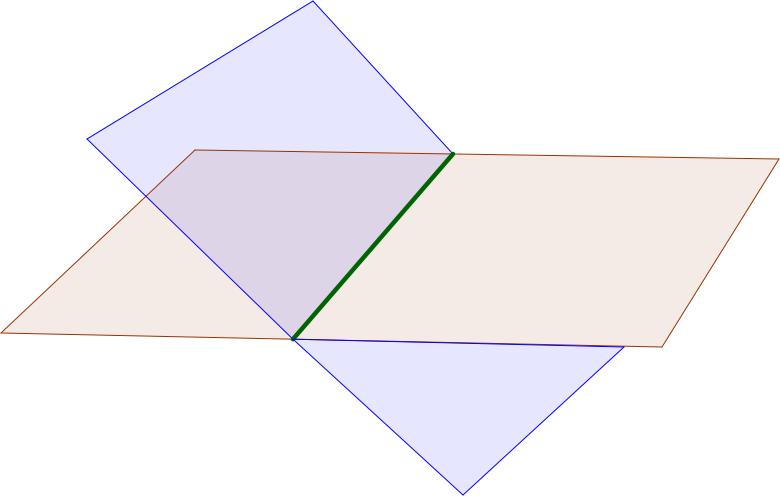
\includegraphics[scale=0.5]{tvaplan.png}
\end{center}
\newpage
Vi kan lägga till en ekvation:
\[
    \begin{cases}
        x_1 - 2x_2 + x_3 = 0\\
        2x_2 - 8x_3 = -8\\
        4x_1 + 5x_2 + 9x_3 = 9
    \end{cases}
\]
\begin{elimination}[1]{3}{1.75em}{1.1}
\step
{
    1 & -2 & 1 & 0\\
    0 & 2 & -8 & 8\\
    4 & 5 & 9 & 9
}
{
    \\
    \\
}
\step
{
    1 & 0 & 0 & 29\\
    0 & 1 & 0 & 16 \\
    0 & 0 & 1 & 3
}
{
    \\
    \\
}
\end{elimination}
Tolkningen blir tre plan och lösningen blir skärningspunkten mellan dessa.
\end{document}